
% Default to the notebook output style

    


% Inherit from the specified cell style.




    
\documentclass[11pt]{article}

    
    
    \usepackage[T1]{fontenc}
    % Nicer default font (+ math font) than Computer Modern for most use cases
    \usepackage{mathpazo}

    % Basic figure setup, for now with no caption control since it's done
    % automatically by Pandoc (which extracts ![](path) syntax from Markdown).
    \usepackage{graphicx}
    % We will generate all images so they have a width \maxwidth. This means
    % that they will get their normal width if they fit onto the page, but
    % are scaled down if they would overflow the margins.
    \makeatletter
    \def\maxwidth{\ifdim\Gin@nat@width>\linewidth\linewidth
    \else\Gin@nat@width\fi}
    \makeatother
    \let\Oldincludegraphics\includegraphics
    % Set max figure width to be 80% of text width, for now hardcoded.
    \renewcommand{\includegraphics}[1]{\Oldincludegraphics[width=.8\maxwidth]{#1}}
    % Ensure that by default, figures have no caption (until we provide a
    % proper Figure object with a Caption API and a way to capture that
    % in the conversion process - todo).
    \usepackage{caption}
    \DeclareCaptionLabelFormat{nolabel}{}
    \captionsetup{labelformat=nolabel}

    \usepackage{adjustbox} % Used to constrain images to a maximum size 
    \usepackage{xcolor} % Allow colors to be defined
    \usepackage{enumerate} % Needed for markdown enumerations to work
    \usepackage{geometry} % Used to adjust the document margins
    \usepackage{amsmath} % Equations
    \usepackage{amssymb} % Equations
    \usepackage{textcomp} % defines textquotesingle
    % Hack from http://tex.stackexchange.com/a/47451/13684:
    \AtBeginDocument{%
        \def\PYZsq{\textquotesingle}% Upright quotes in Pygmentized code
    }
    \usepackage{upquote} % Upright quotes for verbatim code
    \usepackage{eurosym} % defines \euro
    \usepackage[mathletters]{ucs} % Extended unicode (utf-8) support
    \usepackage[utf8x]{inputenc} % Allow utf-8 characters in the tex document
    \usepackage{fancyvrb} % verbatim replacement that allows latex
    \usepackage{grffile} % extends the file name processing of package graphics 
                         % to support a larger range 
    % The hyperref package gives us a pdf with properly built
    % internal navigation ('pdf bookmarks' for the table of contents,
    % internal cross-reference links, web links for URLs, etc.)
    \usepackage{hyperref}
    \usepackage{longtable} % longtable support required by pandoc >1.10
    \usepackage{booktabs}  % table support for pandoc > 1.12.2
    \usepackage[inline]{enumitem} % IRkernel/repr support (it uses the enumerate* environment)
    \usepackage[normalem]{ulem} % ulem is needed to support strikethroughs (\sout)
                                % normalem makes italics be italics, not underlines
    

    
    
    % Colors for the hyperref package
    \definecolor{urlcolor}{rgb}{0,.145,.698}
    \definecolor{linkcolor}{rgb}{.71,0.21,0.01}
    \definecolor{citecolor}{rgb}{.12,.54,.11}

    % ANSI colors
    \definecolor{ansi-black}{HTML}{3E424D}
    \definecolor{ansi-black-intense}{HTML}{282C36}
    \definecolor{ansi-red}{HTML}{E75C58}
    \definecolor{ansi-red-intense}{HTML}{B22B31}
    \definecolor{ansi-green}{HTML}{00A250}
    \definecolor{ansi-green-intense}{HTML}{007427}
    \definecolor{ansi-yellow}{HTML}{DDB62B}
    \definecolor{ansi-yellow-intense}{HTML}{B27D12}
    \definecolor{ansi-blue}{HTML}{208FFB}
    \definecolor{ansi-blue-intense}{HTML}{0065CA}
    \definecolor{ansi-magenta}{HTML}{D160C4}
    \definecolor{ansi-magenta-intense}{HTML}{A03196}
    \definecolor{ansi-cyan}{HTML}{60C6C8}
    \definecolor{ansi-cyan-intense}{HTML}{258F8F}
    \definecolor{ansi-white}{HTML}{C5C1B4}
    \definecolor{ansi-white-intense}{HTML}{A1A6B2}

    % commands and environments needed by pandoc snippets
    % extracted from the output of `pandoc -s`
    \providecommand{\tightlist}{%
      \setlength{\itemsep}{0pt}\setlength{\parskip}{0pt}}
    \DefineVerbatimEnvironment{Highlighting}{Verbatim}{commandchars=\\\{\}}
    % Add ',fontsize=\small' for more characters per line
    \newenvironment{Shaded}{}{}
    \newcommand{\KeywordTok}[1]{\textcolor[rgb]{0.00,0.44,0.13}{\textbf{{#1}}}}
    \newcommand{\DataTypeTok}[1]{\textcolor[rgb]{0.56,0.13,0.00}{{#1}}}
    \newcommand{\DecValTok}[1]{\textcolor[rgb]{0.25,0.63,0.44}{{#1}}}
    \newcommand{\BaseNTok}[1]{\textcolor[rgb]{0.25,0.63,0.44}{{#1}}}
    \newcommand{\FloatTok}[1]{\textcolor[rgb]{0.25,0.63,0.44}{{#1}}}
    \newcommand{\CharTok}[1]{\textcolor[rgb]{0.25,0.44,0.63}{{#1}}}
    \newcommand{\StringTok}[1]{\textcolor[rgb]{0.25,0.44,0.63}{{#1}}}
    \newcommand{\CommentTok}[1]{\textcolor[rgb]{0.38,0.63,0.69}{\textit{{#1}}}}
    \newcommand{\OtherTok}[1]{\textcolor[rgb]{0.00,0.44,0.13}{{#1}}}
    \newcommand{\AlertTok}[1]{\textcolor[rgb]{1.00,0.00,0.00}{\textbf{{#1}}}}
    \newcommand{\FunctionTok}[1]{\textcolor[rgb]{0.02,0.16,0.49}{{#1}}}
    \newcommand{\RegionMarkerTok}[1]{{#1}}
    \newcommand{\ErrorTok}[1]{\textcolor[rgb]{1.00,0.00,0.00}{\textbf{{#1}}}}
    \newcommand{\NormalTok}[1]{{#1}}
    
    % Additional commands for more recent versions of Pandoc
    \newcommand{\ConstantTok}[1]{\textcolor[rgb]{0.53,0.00,0.00}{{#1}}}
    \newcommand{\SpecialCharTok}[1]{\textcolor[rgb]{0.25,0.44,0.63}{{#1}}}
    \newcommand{\VerbatimStringTok}[1]{\textcolor[rgb]{0.25,0.44,0.63}{{#1}}}
    \newcommand{\SpecialStringTok}[1]{\textcolor[rgb]{0.73,0.40,0.53}{{#1}}}
    \newcommand{\ImportTok}[1]{{#1}}
    \newcommand{\DocumentationTok}[1]{\textcolor[rgb]{0.73,0.13,0.13}{\textit{{#1}}}}
    \newcommand{\AnnotationTok}[1]{\textcolor[rgb]{0.38,0.63,0.69}{\textbf{\textit{{#1}}}}}
    \newcommand{\CommentVarTok}[1]{\textcolor[rgb]{0.38,0.63,0.69}{\textbf{\textit{{#1}}}}}
    \newcommand{\VariableTok}[1]{\textcolor[rgb]{0.10,0.09,0.49}{{#1}}}
    \newcommand{\ControlFlowTok}[1]{\textcolor[rgb]{0.00,0.44,0.13}{\textbf{{#1}}}}
    \newcommand{\OperatorTok}[1]{\textcolor[rgb]{0.40,0.40,0.40}{{#1}}}
    \newcommand{\BuiltInTok}[1]{{#1}}
    \newcommand{\ExtensionTok}[1]{{#1}}
    \newcommand{\PreprocessorTok}[1]{\textcolor[rgb]{0.74,0.48,0.00}{{#1}}}
    \newcommand{\AttributeTok}[1]{\textcolor[rgb]{0.49,0.56,0.16}{{#1}}}
    \newcommand{\InformationTok}[1]{\textcolor[rgb]{0.38,0.63,0.69}{\textbf{\textit{{#1}}}}}
    \newcommand{\WarningTok}[1]{\textcolor[rgb]{0.38,0.63,0.69}{\textbf{\textit{{#1}}}}}
    
    
    % Define a nice break command that doesn't care if a line doesn't already
    % exist.
    \def\br{\hspace*{\fill} \\* }
    % Math Jax compatability definitions
    \def\gt{>}
    \def\lt{<}
    % Document parameters
    \title{week2}
    
    
    

    % Pygments definitions
    
\makeatletter
\def\PY@reset{\let\PY@it=\relax \let\PY@bf=\relax%
    \let\PY@ul=\relax \let\PY@tc=\relax%
    \let\PY@bc=\relax \let\PY@ff=\relax}
\def\PY@tok#1{\csname PY@tok@#1\endcsname}
\def\PY@toks#1+{\ifx\relax#1\empty\else%
    \PY@tok{#1}\expandafter\PY@toks\fi}
\def\PY@do#1{\PY@bc{\PY@tc{\PY@ul{%
    \PY@it{\PY@bf{\PY@ff{#1}}}}}}}
\def\PY#1#2{\PY@reset\PY@toks#1+\relax+\PY@do{#2}}

\expandafter\def\csname PY@tok@w\endcsname{\def\PY@tc##1{\textcolor[rgb]{0.73,0.73,0.73}{##1}}}
\expandafter\def\csname PY@tok@c\endcsname{\let\PY@it=\textit\def\PY@tc##1{\textcolor[rgb]{0.25,0.50,0.50}{##1}}}
\expandafter\def\csname PY@tok@cp\endcsname{\def\PY@tc##1{\textcolor[rgb]{0.74,0.48,0.00}{##1}}}
\expandafter\def\csname PY@tok@k\endcsname{\let\PY@bf=\textbf\def\PY@tc##1{\textcolor[rgb]{0.00,0.50,0.00}{##1}}}
\expandafter\def\csname PY@tok@kp\endcsname{\def\PY@tc##1{\textcolor[rgb]{0.00,0.50,0.00}{##1}}}
\expandafter\def\csname PY@tok@kt\endcsname{\def\PY@tc##1{\textcolor[rgb]{0.69,0.00,0.25}{##1}}}
\expandafter\def\csname PY@tok@o\endcsname{\def\PY@tc##1{\textcolor[rgb]{0.40,0.40,0.40}{##1}}}
\expandafter\def\csname PY@tok@ow\endcsname{\let\PY@bf=\textbf\def\PY@tc##1{\textcolor[rgb]{0.67,0.13,1.00}{##1}}}
\expandafter\def\csname PY@tok@nb\endcsname{\def\PY@tc##1{\textcolor[rgb]{0.00,0.50,0.00}{##1}}}
\expandafter\def\csname PY@tok@nf\endcsname{\def\PY@tc##1{\textcolor[rgb]{0.00,0.00,1.00}{##1}}}
\expandafter\def\csname PY@tok@nc\endcsname{\let\PY@bf=\textbf\def\PY@tc##1{\textcolor[rgb]{0.00,0.00,1.00}{##1}}}
\expandafter\def\csname PY@tok@nn\endcsname{\let\PY@bf=\textbf\def\PY@tc##1{\textcolor[rgb]{0.00,0.00,1.00}{##1}}}
\expandafter\def\csname PY@tok@ne\endcsname{\let\PY@bf=\textbf\def\PY@tc##1{\textcolor[rgb]{0.82,0.25,0.23}{##1}}}
\expandafter\def\csname PY@tok@nv\endcsname{\def\PY@tc##1{\textcolor[rgb]{0.10,0.09,0.49}{##1}}}
\expandafter\def\csname PY@tok@no\endcsname{\def\PY@tc##1{\textcolor[rgb]{0.53,0.00,0.00}{##1}}}
\expandafter\def\csname PY@tok@nl\endcsname{\def\PY@tc##1{\textcolor[rgb]{0.63,0.63,0.00}{##1}}}
\expandafter\def\csname PY@tok@ni\endcsname{\let\PY@bf=\textbf\def\PY@tc##1{\textcolor[rgb]{0.60,0.60,0.60}{##1}}}
\expandafter\def\csname PY@tok@na\endcsname{\def\PY@tc##1{\textcolor[rgb]{0.49,0.56,0.16}{##1}}}
\expandafter\def\csname PY@tok@nt\endcsname{\let\PY@bf=\textbf\def\PY@tc##1{\textcolor[rgb]{0.00,0.50,0.00}{##1}}}
\expandafter\def\csname PY@tok@nd\endcsname{\def\PY@tc##1{\textcolor[rgb]{0.67,0.13,1.00}{##1}}}
\expandafter\def\csname PY@tok@s\endcsname{\def\PY@tc##1{\textcolor[rgb]{0.73,0.13,0.13}{##1}}}
\expandafter\def\csname PY@tok@sd\endcsname{\let\PY@it=\textit\def\PY@tc##1{\textcolor[rgb]{0.73,0.13,0.13}{##1}}}
\expandafter\def\csname PY@tok@si\endcsname{\let\PY@bf=\textbf\def\PY@tc##1{\textcolor[rgb]{0.73,0.40,0.53}{##1}}}
\expandafter\def\csname PY@tok@se\endcsname{\let\PY@bf=\textbf\def\PY@tc##1{\textcolor[rgb]{0.73,0.40,0.13}{##1}}}
\expandafter\def\csname PY@tok@sr\endcsname{\def\PY@tc##1{\textcolor[rgb]{0.73,0.40,0.53}{##1}}}
\expandafter\def\csname PY@tok@ss\endcsname{\def\PY@tc##1{\textcolor[rgb]{0.10,0.09,0.49}{##1}}}
\expandafter\def\csname PY@tok@sx\endcsname{\def\PY@tc##1{\textcolor[rgb]{0.00,0.50,0.00}{##1}}}
\expandafter\def\csname PY@tok@m\endcsname{\def\PY@tc##1{\textcolor[rgb]{0.40,0.40,0.40}{##1}}}
\expandafter\def\csname PY@tok@gh\endcsname{\let\PY@bf=\textbf\def\PY@tc##1{\textcolor[rgb]{0.00,0.00,0.50}{##1}}}
\expandafter\def\csname PY@tok@gu\endcsname{\let\PY@bf=\textbf\def\PY@tc##1{\textcolor[rgb]{0.50,0.00,0.50}{##1}}}
\expandafter\def\csname PY@tok@gd\endcsname{\def\PY@tc##1{\textcolor[rgb]{0.63,0.00,0.00}{##1}}}
\expandafter\def\csname PY@tok@gi\endcsname{\def\PY@tc##1{\textcolor[rgb]{0.00,0.63,0.00}{##1}}}
\expandafter\def\csname PY@tok@gr\endcsname{\def\PY@tc##1{\textcolor[rgb]{1.00,0.00,0.00}{##1}}}
\expandafter\def\csname PY@tok@ge\endcsname{\let\PY@it=\textit}
\expandafter\def\csname PY@tok@gs\endcsname{\let\PY@bf=\textbf}
\expandafter\def\csname PY@tok@gp\endcsname{\let\PY@bf=\textbf\def\PY@tc##1{\textcolor[rgb]{0.00,0.00,0.50}{##1}}}
\expandafter\def\csname PY@tok@go\endcsname{\def\PY@tc##1{\textcolor[rgb]{0.53,0.53,0.53}{##1}}}
\expandafter\def\csname PY@tok@gt\endcsname{\def\PY@tc##1{\textcolor[rgb]{0.00,0.27,0.87}{##1}}}
\expandafter\def\csname PY@tok@err\endcsname{\def\PY@bc##1{\setlength{\fboxsep}{0pt}\fcolorbox[rgb]{1.00,0.00,0.00}{1,1,1}{\strut ##1}}}
\expandafter\def\csname PY@tok@kc\endcsname{\let\PY@bf=\textbf\def\PY@tc##1{\textcolor[rgb]{0.00,0.50,0.00}{##1}}}
\expandafter\def\csname PY@tok@kd\endcsname{\let\PY@bf=\textbf\def\PY@tc##1{\textcolor[rgb]{0.00,0.50,0.00}{##1}}}
\expandafter\def\csname PY@tok@kn\endcsname{\let\PY@bf=\textbf\def\PY@tc##1{\textcolor[rgb]{0.00,0.50,0.00}{##1}}}
\expandafter\def\csname PY@tok@kr\endcsname{\let\PY@bf=\textbf\def\PY@tc##1{\textcolor[rgb]{0.00,0.50,0.00}{##1}}}
\expandafter\def\csname PY@tok@bp\endcsname{\def\PY@tc##1{\textcolor[rgb]{0.00,0.50,0.00}{##1}}}
\expandafter\def\csname PY@tok@fm\endcsname{\def\PY@tc##1{\textcolor[rgb]{0.00,0.00,1.00}{##1}}}
\expandafter\def\csname PY@tok@vc\endcsname{\def\PY@tc##1{\textcolor[rgb]{0.10,0.09,0.49}{##1}}}
\expandafter\def\csname PY@tok@vg\endcsname{\def\PY@tc##1{\textcolor[rgb]{0.10,0.09,0.49}{##1}}}
\expandafter\def\csname PY@tok@vi\endcsname{\def\PY@tc##1{\textcolor[rgb]{0.10,0.09,0.49}{##1}}}
\expandafter\def\csname PY@tok@vm\endcsname{\def\PY@tc##1{\textcolor[rgb]{0.10,0.09,0.49}{##1}}}
\expandafter\def\csname PY@tok@sa\endcsname{\def\PY@tc##1{\textcolor[rgb]{0.73,0.13,0.13}{##1}}}
\expandafter\def\csname PY@tok@sb\endcsname{\def\PY@tc##1{\textcolor[rgb]{0.73,0.13,0.13}{##1}}}
\expandafter\def\csname PY@tok@sc\endcsname{\def\PY@tc##1{\textcolor[rgb]{0.73,0.13,0.13}{##1}}}
\expandafter\def\csname PY@tok@dl\endcsname{\def\PY@tc##1{\textcolor[rgb]{0.73,0.13,0.13}{##1}}}
\expandafter\def\csname PY@tok@s2\endcsname{\def\PY@tc##1{\textcolor[rgb]{0.73,0.13,0.13}{##1}}}
\expandafter\def\csname PY@tok@sh\endcsname{\def\PY@tc##1{\textcolor[rgb]{0.73,0.13,0.13}{##1}}}
\expandafter\def\csname PY@tok@s1\endcsname{\def\PY@tc##1{\textcolor[rgb]{0.73,0.13,0.13}{##1}}}
\expandafter\def\csname PY@tok@mb\endcsname{\def\PY@tc##1{\textcolor[rgb]{0.40,0.40,0.40}{##1}}}
\expandafter\def\csname PY@tok@mf\endcsname{\def\PY@tc##1{\textcolor[rgb]{0.40,0.40,0.40}{##1}}}
\expandafter\def\csname PY@tok@mh\endcsname{\def\PY@tc##1{\textcolor[rgb]{0.40,0.40,0.40}{##1}}}
\expandafter\def\csname PY@tok@mi\endcsname{\def\PY@tc##1{\textcolor[rgb]{0.40,0.40,0.40}{##1}}}
\expandafter\def\csname PY@tok@il\endcsname{\def\PY@tc##1{\textcolor[rgb]{0.40,0.40,0.40}{##1}}}
\expandafter\def\csname PY@tok@mo\endcsname{\def\PY@tc##1{\textcolor[rgb]{0.40,0.40,0.40}{##1}}}
\expandafter\def\csname PY@tok@ch\endcsname{\let\PY@it=\textit\def\PY@tc##1{\textcolor[rgb]{0.25,0.50,0.50}{##1}}}
\expandafter\def\csname PY@tok@cm\endcsname{\let\PY@it=\textit\def\PY@tc##1{\textcolor[rgb]{0.25,0.50,0.50}{##1}}}
\expandafter\def\csname PY@tok@cpf\endcsname{\let\PY@it=\textit\def\PY@tc##1{\textcolor[rgb]{0.25,0.50,0.50}{##1}}}
\expandafter\def\csname PY@tok@c1\endcsname{\let\PY@it=\textit\def\PY@tc##1{\textcolor[rgb]{0.25,0.50,0.50}{##1}}}
\expandafter\def\csname PY@tok@cs\endcsname{\let\PY@it=\textit\def\PY@tc##1{\textcolor[rgb]{0.25,0.50,0.50}{##1}}}

\def\PYZbs{\char`\\}
\def\PYZus{\char`\_}
\def\PYZob{\char`\{}
\def\PYZcb{\char`\}}
\def\PYZca{\char`\^}
\def\PYZam{\char`\&}
\def\PYZlt{\char`\<}
\def\PYZgt{\char`\>}
\def\PYZsh{\char`\#}
\def\PYZpc{\char`\%}
\def\PYZdl{\char`\$}
\def\PYZhy{\char`\-}
\def\PYZsq{\char`\'}
\def\PYZdq{\char`\"}
\def\PYZti{\char`\~}
% for compatibility with earlier versions
\def\PYZat{@}
\def\PYZlb{[}
\def\PYZrb{]}
\makeatother


    % Exact colors from NB
    \definecolor{incolor}{rgb}{0.0, 0.0, 0.5}
    \definecolor{outcolor}{rgb}{0.545, 0.0, 0.0}



    
    % Prevent overflowing lines due to hard-to-break entities
    \sloppy 
    % Setup hyperref package
    \hypersetup{
      breaklinks=true,  % so long urls are correctly broken across lines
      colorlinks=true,
      urlcolor=urlcolor,
      linkcolor=linkcolor,
      citecolor=citecolor,
      }
    % Slightly bigger margins than the latex defaults
    
    \geometry{verbose,tmargin=1in,bmargin=1in,lmargin=1in,rmargin=1in}
    
    

    \begin{document}
    
    
    \maketitle
    
    

    
    \subsection{Additional Readings and
Resources}\label{additional-readings-and-resources}

Design:

\begin{itemize}
\tightlist
\item
  The Visual Display of Quantitative Information by Edward Tufte
\item
  Envisioning Information by Edward Tufte
\item
  Visual Explanations: Images and Quantities, Evidence and Narrative by
  Edward Tufte
\end{itemize}

Color:

\begin{itemize}
\tightlist
\item
  Information Visualization: Perception for Design by Colin Ware
\end{itemize}

    \subsection{Key phrases and Concepts}\label{key-phrases-and-concepts}

\begin{itemize}
\tightlist
\item
  Data variables: nominal, ordinal, and quantitative; discrete v.
  continuous; dependent v. independent
\item
  The perceptual accuracy of how different chart elements represent data
  variables
\item
  How glyphs represent multiple dimensions of individual data items, how
  parallel coordinates plot data over many dimensions, and how
  streamgraphs improve on stacked bar charts
\item
  Chartjunk, the data-ink ratio, and other design rules
\item
  Hue, saturation, value, and other ways of thinking about color
\end{itemize}

    \subsection{Introduction}\label{introduction}

We can use \href{https://www.tableau.com/}{Tableau} to visualize dan
analyze data. Tableau has easy navigation, for example, we can easily
found a "Show More" button to choose proper graph to visualize
correspondent data.

    \subsection{Data Visualization
Framework}\label{data-visualization-framework}

There is a framework to help us and simplify our understanding of how
data visualization work. The \textbf{data visualization framework} can
be seen in an image below:

\begin{figure}
\centering
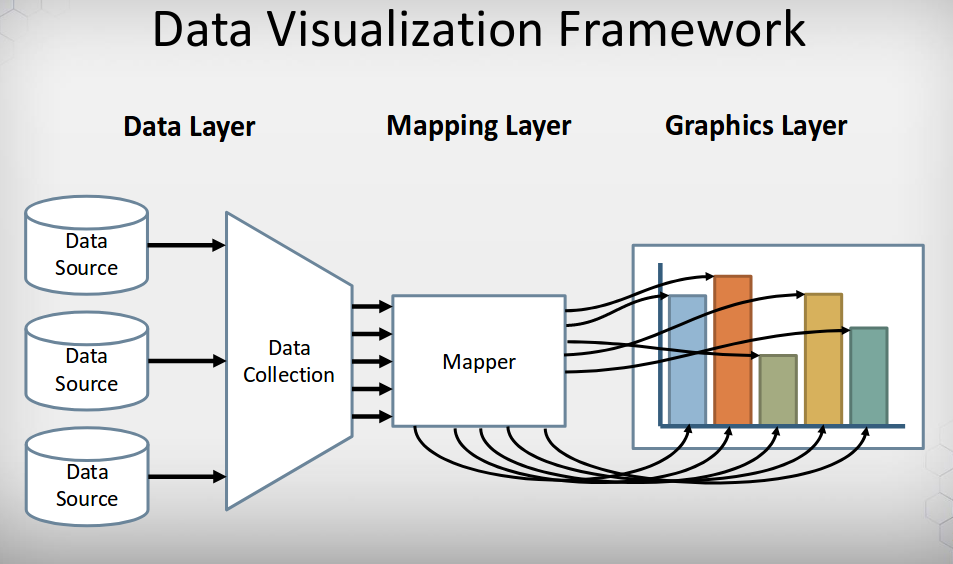
\includegraphics{images/data-visualization-framework.png}
\caption{Data visualization framework}
\end{figure}

\textbf{Data Layer} contains two entities that are data sources and data
collection. Before collecting all data, we need to do preprocessing that
ensuring each data imported in the proper format. After data being
imported, we need to ensure that all data stored in the best possible
structure. In the case of a database, we can maintenance relation
between data as database indexes, so will increase retrieval time. After
data storing problem being solved, we can do such optimization to
enhance our storage. By doing data analysis, we can decide the quality
of data we have collected. The task of data analysis included:
inspecting, cleansing, and transforming. The goal of data analysis is
reduced noise in our data collection, by removing or transforming.
Another crucial optimization is data aggregation which has a significant
impact on retrieval performance of our data collection. The task of data
aggregation included: classification, clustering, etc.

\textbf{Mapping Layer} is a complicated layer which has robust
implementation of linear algebra and computer graphics algorithms. In
this layer, we working on how to associating appropriate geometry with
data channels. For example, in the case to represent clusters of data,
we need to associate size of cluster into area of circle.

\textbf{Graphics layer} has a robust implementation of computer graphics
algorithms and user interaction. The main objective of this layer is to
produce geometry calculation from mapping layer into a displayable image
on the computer screen. In the case of interactive visualization, we
need to ensure that any given input processed correctly to produce
expected effect on graphical representation of our data.

    \subsection{Data Types}\label{data-types}

There are four types of discrete data:

\begin{enumerate}
\def\labelenumi{\arabic{enumi}.}
\tightlist
\item
  Ordinal is type of ordered data defined by range. For example: Small
  and large.
\item
  Quantitative is type of ordered data defined by step. For example: 1,
  2, 3, 4, ...
\item
  Nominal is type of unordered data defined by label. For example:
  Shapes (circle / rectangle) and gender (male / female).
\item
  Category is type of unordered data defined by group. For example:
  Social ages (young / old) and nationality.
\end{enumerate}

There are two types of continous data:

\begin{enumerate}
\def\labelenumi{\arabic{enumi}.}
\tightlist
\item
  Fields is type of ordered data defined by standarized scale. For
  example: Temperature data may defined by Celcius or Kelvin and
  altitude data may defined by minute or degree.
\item
  Cyclic values is type of unordered data defined by perception. For
  example: Direction data may indicate by north, south, east, and west
  or clock.
\end{enumerate}

An image below describes briefly each type of data with a good example:

\begin{figure}
\centering
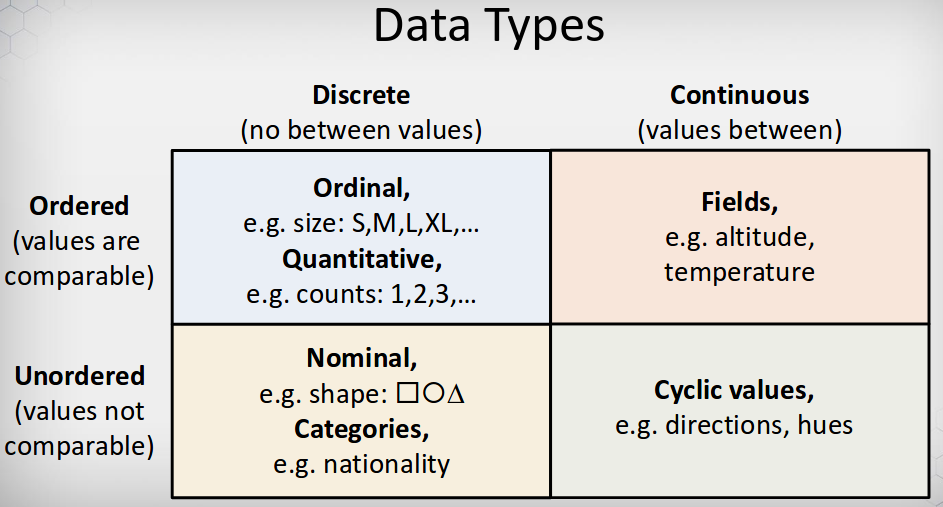
\includegraphics{images/data-type.png}
\caption{data\_type}
\end{figure}

    \subsection{Data as Variable}\label{data-as-variable}

There are two type of data as variable:

\begin{itemize}
\tightlist
\item
  Independent variable is variable which desribed by itself and not
  changed when another value changed.
\item
  Dependent variable is variable which described by another variable.
  For example, y as dependent variable and x as independent variable,
  then value of y is defined by change of x values.
\end{itemize}

An image below describes briefly how data looked in three points of
views: science, database, and data warehouse.

\begin{figure}
\centering
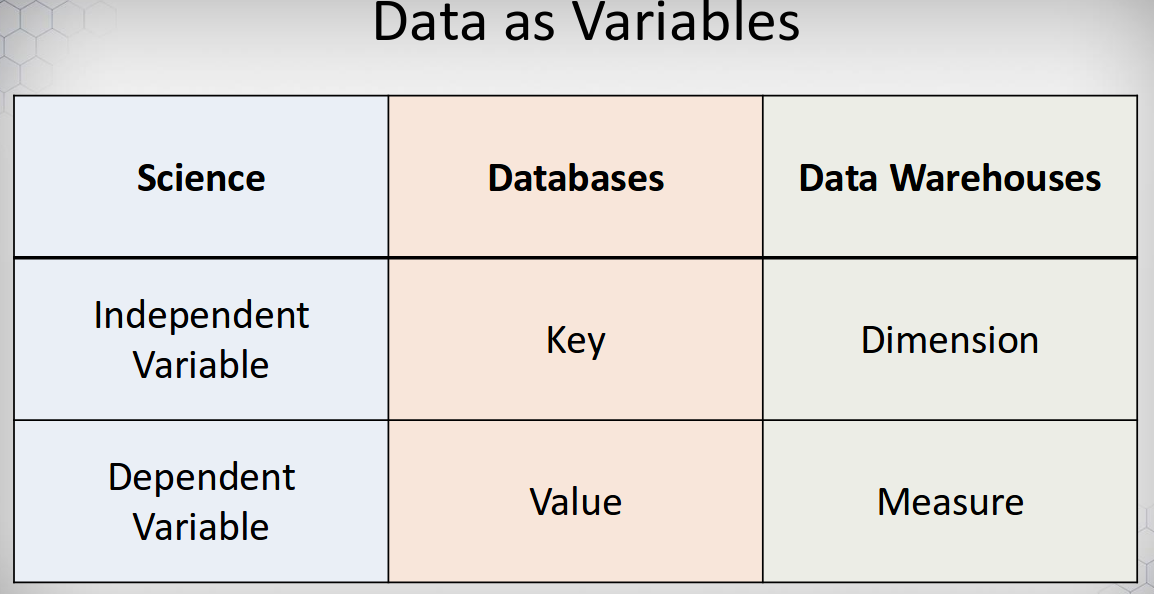
\includegraphics{images/data-variable.png}
\caption{data\_variables}
\end{figure}

    \subsection{Mapping}\label{mapping}

As explained in the mapping layer, the mapping process mainly focused on
produce proper geometry primitive to the corresponding data channel. It
is very important to know which best geometry to represent correspondent
data. Failure in deciding best-suited geometry lead to bad perception
that will influence the quality of interpretation and conclusion.

There are three group of geometry primitives classified by its
dimensions: 1. 1 dimension * Position * Length
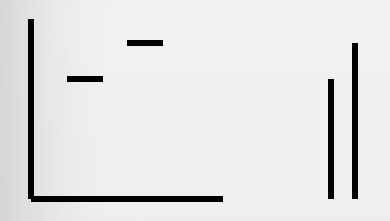
\includegraphics{images/position-length.png} * Angle/Slope
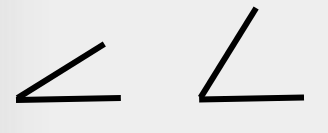
\includegraphics{images/angle.png} 2. 2 dimension * Area

\includegraphics{images/area.png} * Texture * Connection * Containtment
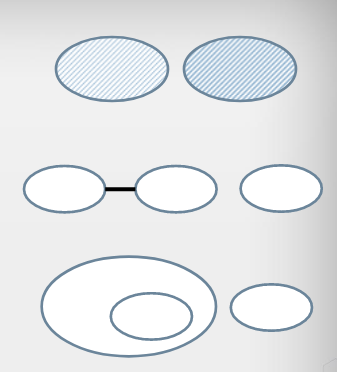
\includegraphics{images/texture-connection-containtment.png} * Shape 3.
3 dimension * Volume * Color/Density
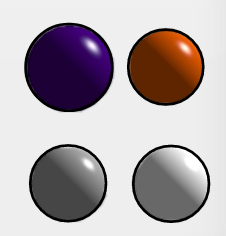
\includegraphics{images/volume-density.png} * Saturation * Hue

Below are three list of suited geometry primitives for three commonly
used data types (quantitative, ordinal, and nominal) ordered by
\textbf{perceptual accuary}.

\begin{longtable}[]{@{}lll@{}}
\toprule
quantitative & ordinal & nominal\tabularnewline
\midrule
\endhead
position & position & position\tabularnewline
length & density & hue\tabularnewline
angle & saturation & texture\tabularnewline
slope & hue & connection\tabularnewline
area & texture & containtment\tabularnewline
volume & connection & density\tabularnewline
density & containtment & saturation\tabularnewline
saturation & length & shape\tabularnewline
hue & angle & length\tabularnewline
& slope & angle\tabularnewline
& area & slope\tabularnewline
& volume & area\tabularnewline
& & volume\tabularnewline
\bottomrule
\end{longtable}

    \subsection{Charts}\label{charts}

Data visualization often consist very simple charts, but the success of
data visualization can often depend on how we map our data to the
elements of those charts. Here we discuss some of the simple charts and
describe when we use each of them.

\begin{enumerate}
\def\labelenumi{\arabic{enumi}.}
\tightlist
\item
  Bar chart 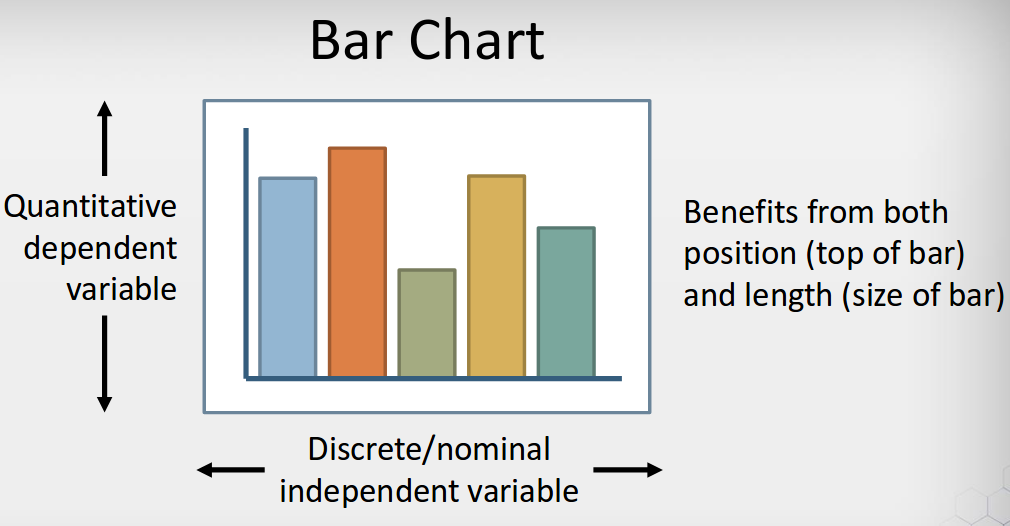
\includegraphics{images/bar.png} 
\item
  Line chart 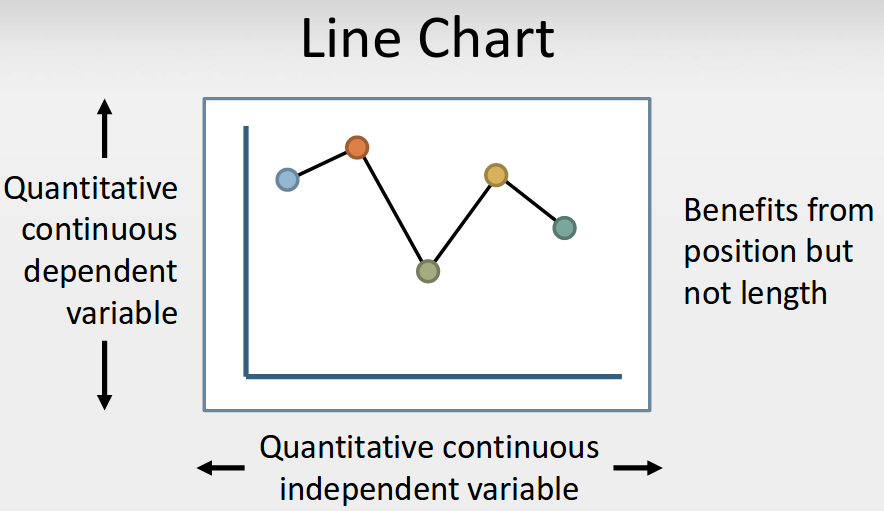
\includegraphics{images/line.png} 
\item
  Scatterplot 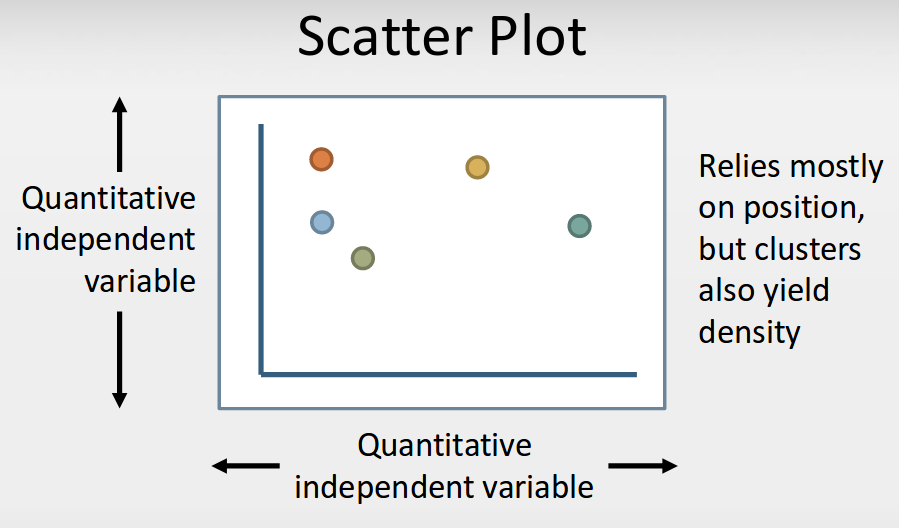
\includegraphics{images/scatter.png}\\
\item
  Gantt chart 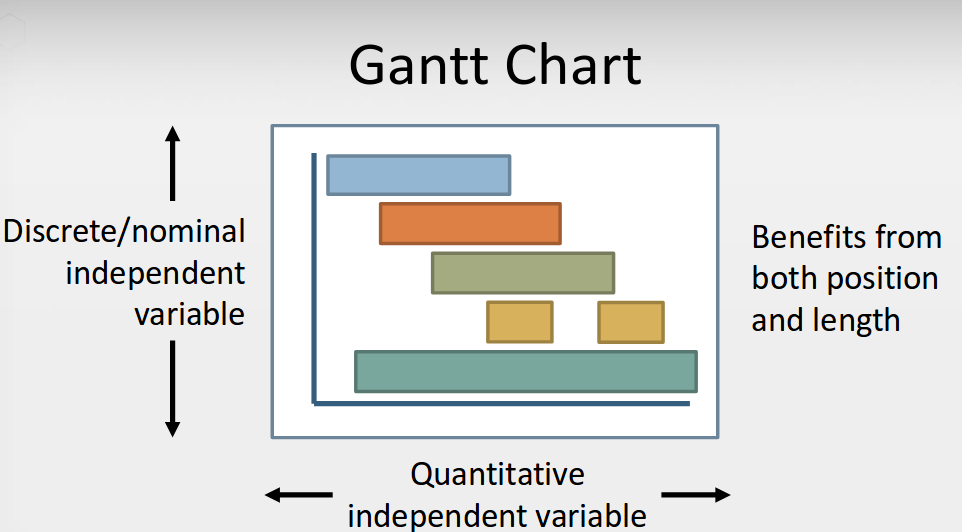
\includegraphics{images/gantt.png}\\
\item
  Table 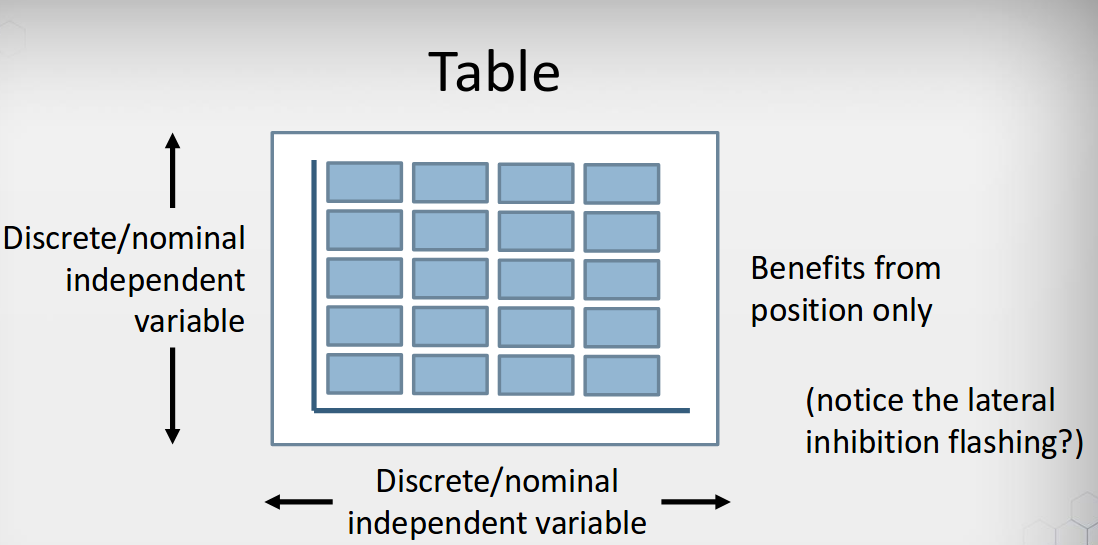
\includegraphics{images/table.png}
\end{enumerate}

We can classify each type of chart by its characteristics:

\begin{figure}
\centering
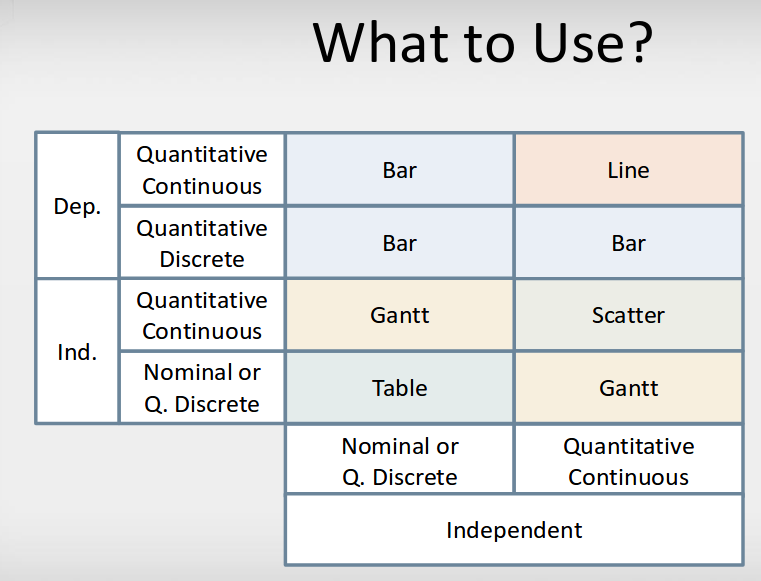
\includegraphics{images/when-use-charts.png}
\caption{when-use-charts}
\end{figure}

    \subsection{Glyphs}\label{glyphs}

Glyphs is any indicators that may encoded as shapes and colors to
represent each kind of data point. For example, to represent a tornado
presentation, we may used length and angle to indicate wind speed and
direction. We may also used hue and shape to indicate density and
coverage such as wind convergence or disvergence is such area. An image
below illustrated use of glyphs in various charts:

\begin{figure}
\centering
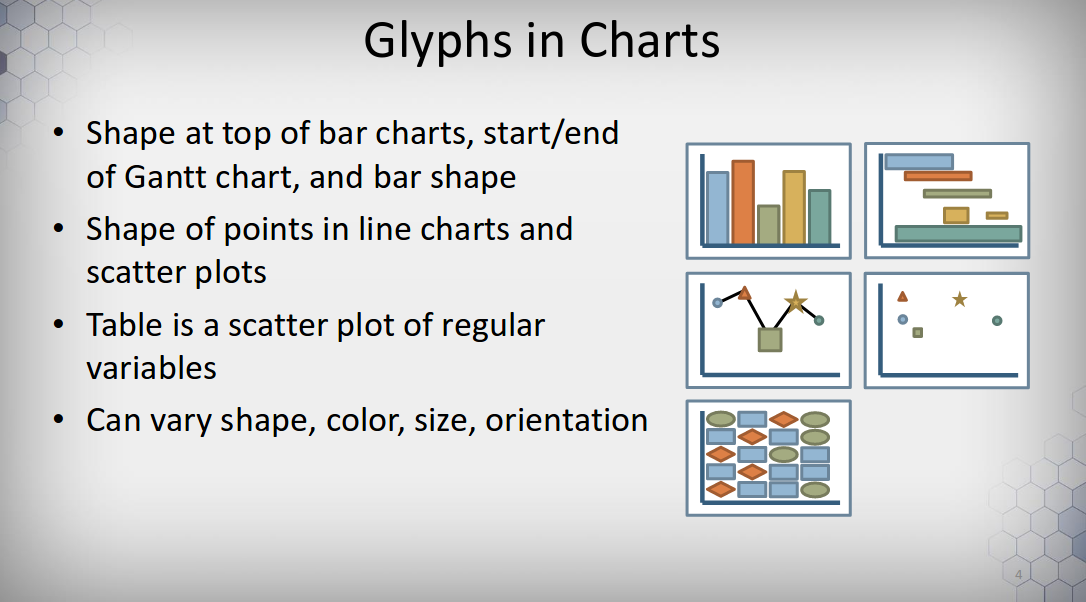
\includegraphics{images/glyphs-in-charts.png}
\caption{glyphs}
\end{figure}

Furthermore, we can use glyphs to show data attributes in the charts or
other visualization. A very common practical example of using glyphs is
visualizing standart deviation and variances in sample data as shown in
image below:

\begin{figure}
\centering
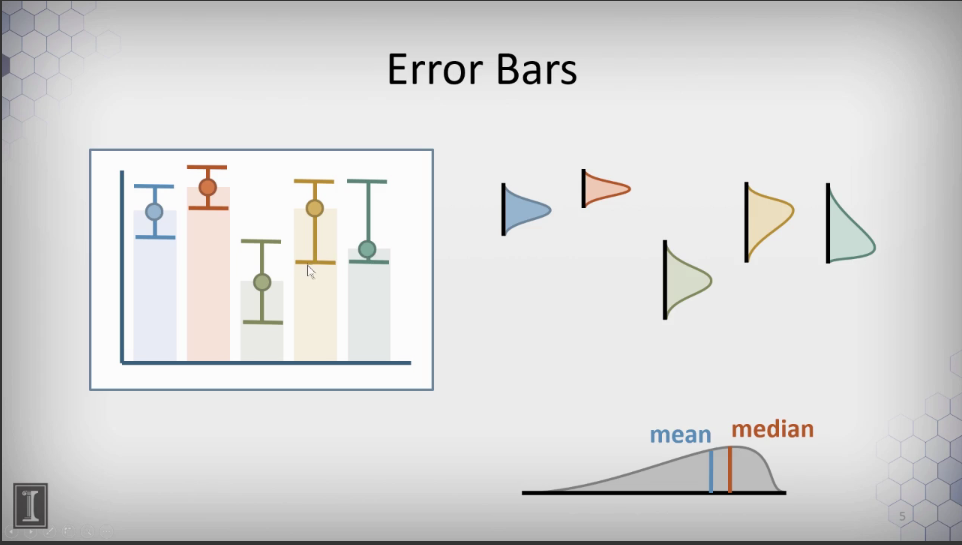
\includegraphics{images/glyphs-standart-deviation.png}
\caption{standart deviation}
\end{figure}

Glyphs can be used in presentation visualization. Heatmap is an example
presentation which used colorized glyphs on the map. Different group or
individual might be not comfort with the Heatmap representation and
demand for higher accuracy. We can used colorized glyphs as boxes with
various hues in the table visualization. The y and x axes on the table
chart discribe data variables and the glyphs help us to show the
differences between data point.

\begin{figure}
\centering
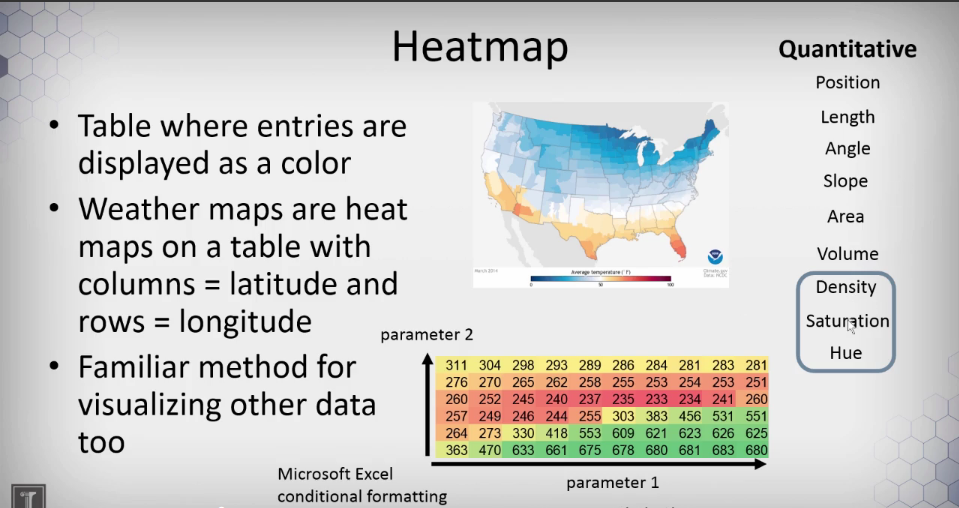
\includegraphics{images/heatmap.png}
\caption{Heatmap}
\end{figure}

In some case, we might want to transform our visualization into more
compact form. We may lost some details and accuary due transformation
into compact form. For example, we may unable to plot detailed graph in
each class of data due limited space. In that case, we doing a trade off
between accuary and classification. An image below show that we can use
glyphs to show differences of life ratio between continent with few
detail about value of life ratio in each class.

\begin{figure}
\centering
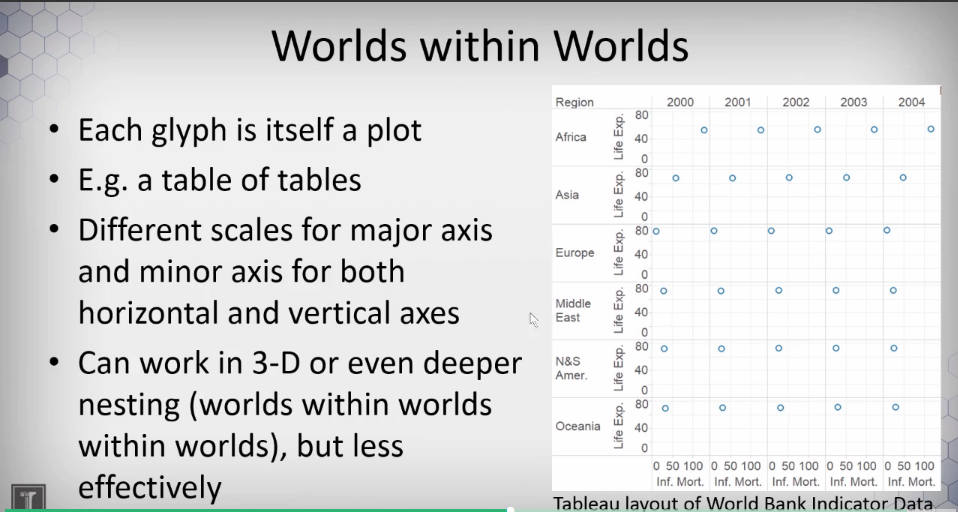
\includegraphics{images/life-ratio.png}
\caption{Life Ratio}
\end{figure}

Glyphs can also represented as features with complex geometry. An image
below is an example of glyphs that represent facial features of lawyers
that tells us some lawyer with bigger face may indicate that some lawyer
have experienced im more cases:

\begin{figure}
\centering
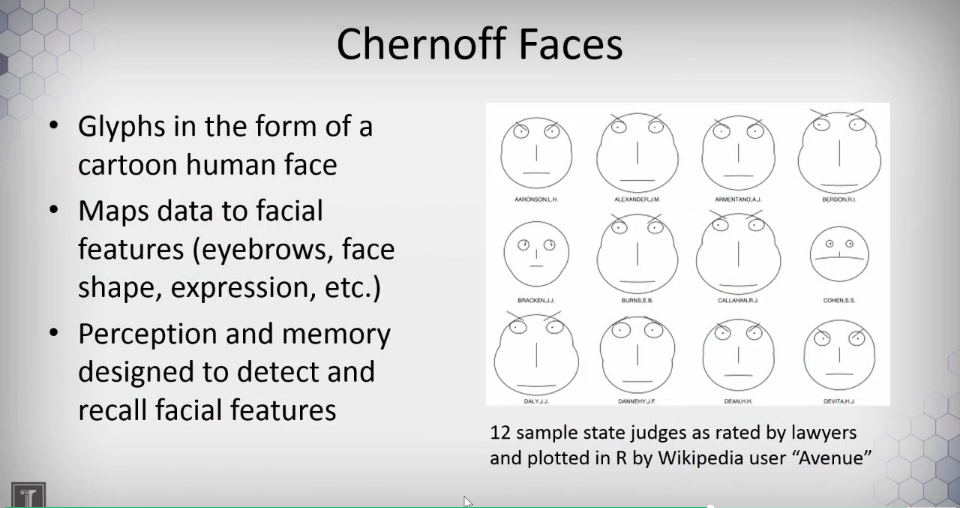
\includegraphics{images/chernoff-faces.png}
\caption{Chernoff Faces}
\end{figure}

    \subsection{Parallel Coordinates}\label{parallel-coordinates}

Parallel coordinates is a visualization technique to visualize
high-dimensional data. This visualization will be very helpful since
most of technology limited in represent high dimensional space as
projection in two dimensional space. The main objective of this
technique is to reveal certain data features, such as
\textbf{collinearity} in high-dimensionality data. The main reason why
we should used this technique is this technique can reduce visualization
complexity due high-dimensionality of data. Below step-by-step how to
construct parallel coordinates of n-dimensions:

\begin{enumerate}
\def\labelenumi{\arabic{enumi}.}
\tightlist
\item
  Create two parallel lines of first two dimensions, for example x and
  y.
\item
  Place each data into each parallel line based on its corresponding
  values. For example, points A(3, 2) and B(4, 3) should be placed at
  y(2, 3) and x(3, 4).
\item
  Draw a lines between two parallel lines corresponding to each data
  points. For example, y(2, 3) and x(3, 4) should became two lines A(3
  to 2) and B(4 to 3).
\item
  Remove every glyph drawn in each parallel line, so there is just lines
  between parallel lines.
\item
  Create one parallel line for next dimension, repeat step 2 until each
  dimension became a parallel line.
\end{enumerate}

The most interesting of parallel coordinate is we can easily detect the
collinearity. As we can see: orange, yellow and green and dark green are
colliniar in x-y plane. Below an example of parallel coordinates of four
dimensional data:

\begin{figure}
\centering
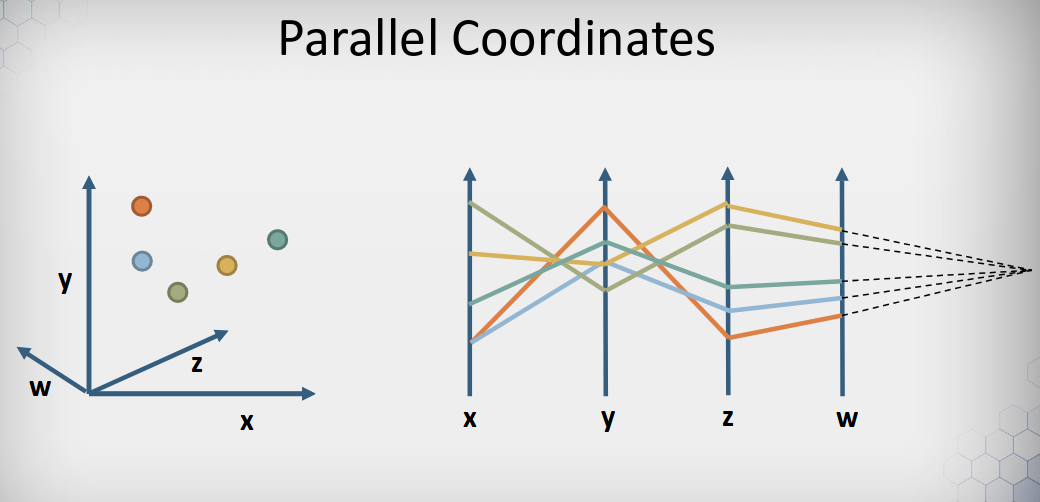
\includegraphics{images/parallel-coordinate.png}
\caption{Parallel coordinate}
\end{figure}

    \subsection{Stacked Graphs}\label{stacked-graphs}

Stacked graphs used when we want to represent accumulated data
(multivariate in same axes). Below type of charts belong to stacked
graph:

\begin{itemize}
\tightlist
\item
  Stacked bar chart
\item
  Relative stacked bar chart
\item
  Pie chart
\item
  Diverging stacked bar chart
\item
  Stacked line graph
\item
  Stacked graph layout
\end{itemize}

In some cases, we need to carefully using stacked bar chart. We already
knew that position more accurate than length in representing
quantitative data. Since stacked bar chart utilize position and length,
we need to prioritize position representation over length. An image
below illustrate how order of position is important.

\begin{figure}
\centering
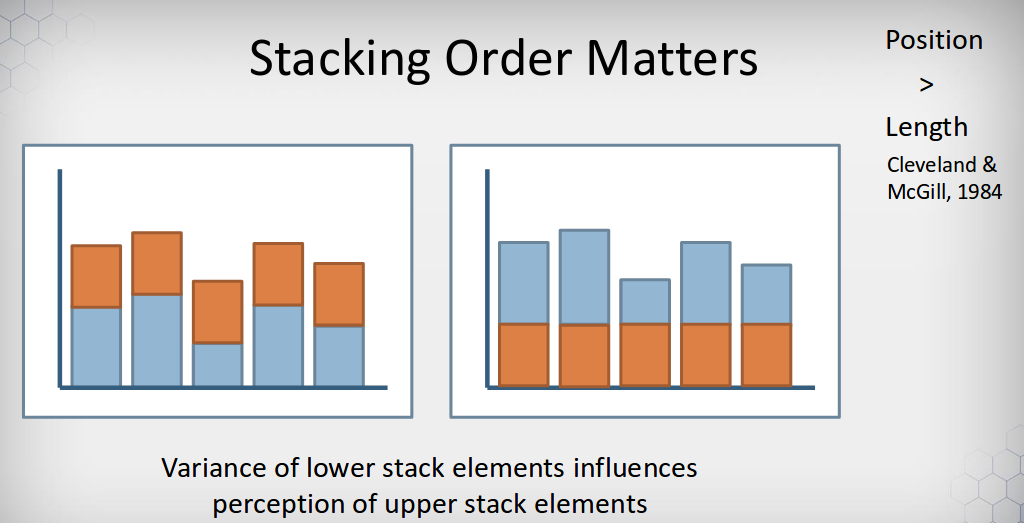
\includegraphics{images/stacked-bar-chart1.png}
\caption{Stacking order}
\end{figure}

Stacked bar chart might be not effective to represent huge accumulated
data. For example, in visualizing multiple stock prices within long time
interval, the stacked graph might be not effective to visualize price
changes. To satisfy that condition, we need to transform stacked bar
chart into stacked graph layout.

\begin{figure}
\centering
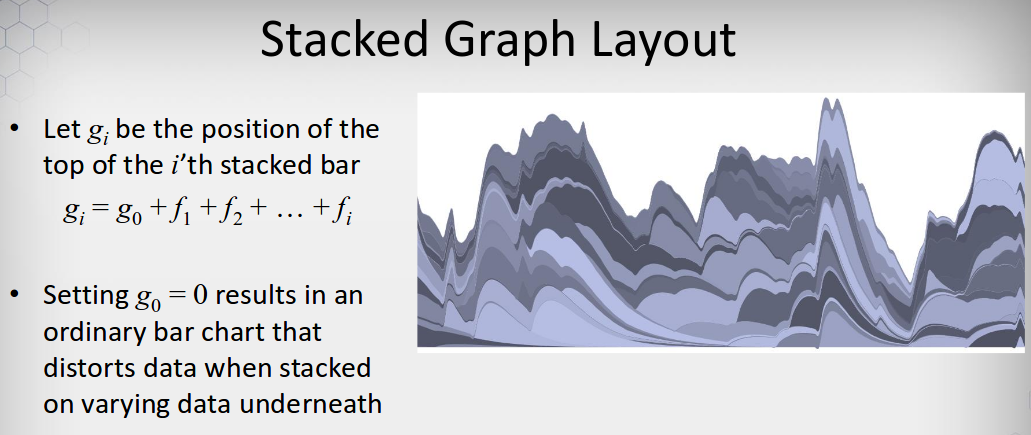
\includegraphics{images/stacked-graph-layout.png}
\caption{Stacked graph layout}
\end{figure}

In order to inspect area or distribution or testing the confidence
interval, we may tranform stacked graph into Themeriver layout

\begin{figure}
\centering
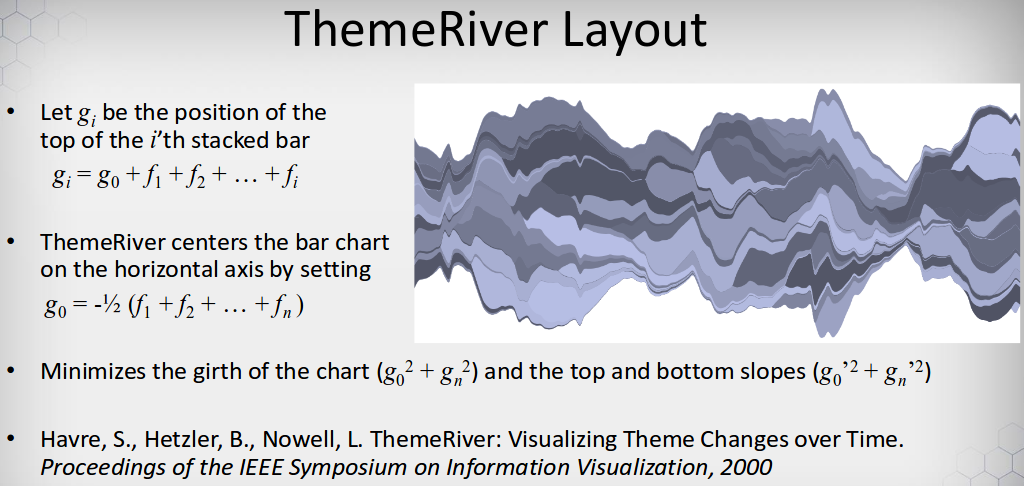
\includegraphics{images/themeriver-layout.png}
\caption{Themeriver Layout}
\end{figure}

In order to do smoothing, if it possible to added some weight, then we
may transfrom themeriver layout into streamgraph layout

\begin{figure}
\centering
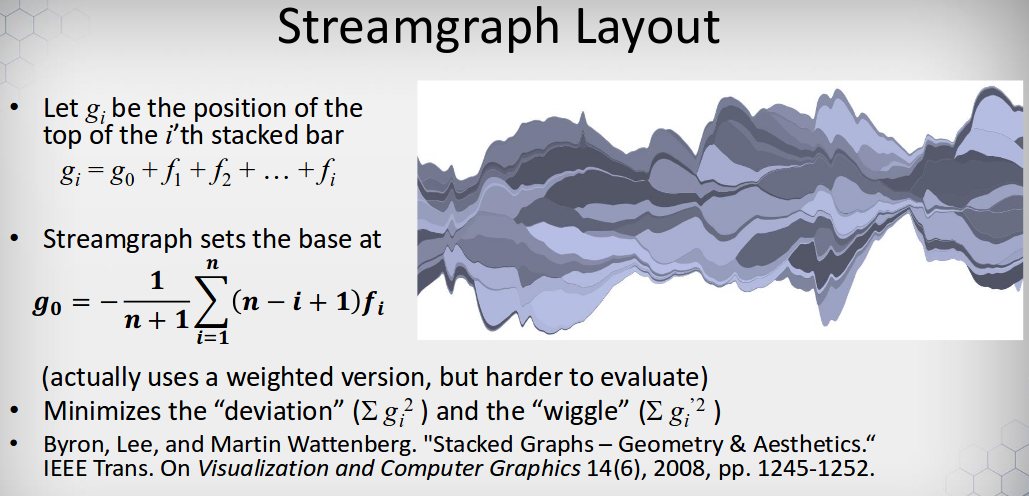
\includegraphics{images/streamgraph-layout.png}
\caption{Streamgraph layout}
\end{figure}

Then, in the case to prioritize position, we may do ordering

\begin{figure}
\centering
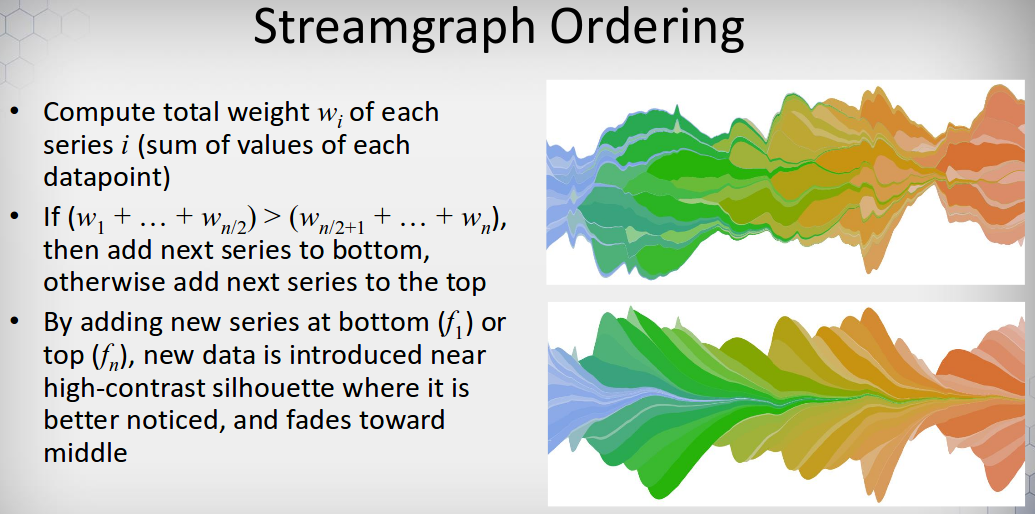
\includegraphics{images/streamgraph-ordering.png}
\caption{Streamgraph ordering}
\end{figure}

    \subsection{Tufte's Design Rules and Using
Color}\label{tuftes-design-rules-and-using-color}

Tufte's Design Rule is one design criteria invented by
\href{https://www.edwardtufte.com/tufte/}{Edward Tufte} which encourage
us to be minimalism in order to visualizing data.

    \subsubsection{Tufte's Design Rules}\label{tuftes-design-rules}

There are some important design rule described by Tufte:

\begin{enumerate}
\def\labelenumi{\arabic{enumi}.}
\tightlist
\item
  Let's data speak: In order to provide reliable data, we must be
  represent the detail of data while guide the audience how to
  interprete data. For example: If there are some missing data, then
  show them with less distraction as possible and making the
  visualization to make audience rely on reasoning to guess how missing
  data should be.
\item
  Try to represent picture as information rather than text: Picture is
  great way to represent data because it has volume, area or length to
  indicate size, color to indicate differentiation and more. By using
  color, we can avoid miss-interpretaion.
\item
  Give annotation: By giving annotation in the data visualization, we
  can inform audience about the detail and supplement information.
\item
  Chart junk: 2D representation may be boring, but 3D representation may
  lead miss-perception.
\item
  The Data-Ink Ratio: When it come to print in the paper, it is good
  idea to follow Tufte's minimalism which try to reduce color as much as
  possible.
\item
  Micro/macro: When it came into detail, we prefer to see micro scales.
  But when it came it the overview, we prefer to see macro scales.
\item
  Information layer: We need to inform audience about any information
  that can be exploited from visualization. For example: We may need to
  create different appearance as different elements such as color and
  shapes.
\item
  Multiple: We need to stay consistent in order to represent some data
  in different cases. For example: We need to stay with exactly same
  chart and glyphs type when represent same measurement method on two
  different machince performance.
\item
  Color: Beware with color combination in visualization because wrong
  color combination may lead miss-interpretation and miss-perception.
\item
  Narrative: A good quality visualization is one that can tells audience
  a story.
\end{enumerate}

    \subsubsection{Using Color}\label{using-color}

\emph{Hue} is defined by angle of color wheel, for example: \(0^0\) is
red, \(60^0\) is yellow, \(120^0\) is green, \(180^0\) is cyan,
\(240^0\) is blue, and \(300^0\) is magenta. \emph{Saturation} is
defined by how far a color from gray. \emph{Value} is defined by how far
a color from black.

Some researches reveal that human can only differentiate between only
five to ten hues (Healy, 1996) and there are only twelve colors (6+6)
recommended by Ward's "Information Visualization".

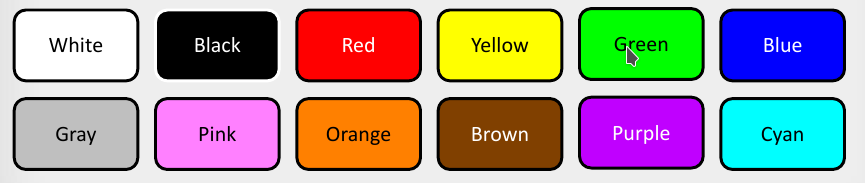
\includegraphics{images/12-colors.png}

In most cases, saturation means giving more details on the object. So
try to add saturated colors for points, strokes, and symbols and add
desaturated colors for bigger or fills larger areas, for example:
desaturated with white to increase luminance. In specific case, such as
plotting bar chart, desaturated color and fills may be better than
saturated colors and fiils.

\emph{Contrast} means differences while in the context of color, it's
deals with hue and optionally for brightness.


    % Add a bibliography block to the postdoc
    
    
    
    \end{document}
